\documentclass[a4paper, 11pt, oneside]{article}

\usepackage[utf8]{inputenc}
\usepackage[T1]{fontenc}
\usepackage[english]{babel}
\usepackage{array}
\usepackage{shortvrb}
\usepackage{listings}
\usepackage[fleqn]{amsmath}
\usepackage{amsfonts}
\usepackage{fullpage}
\usepackage{enumerate}
\usepackage{enumitem}
\usepackage{graphicx}
\usepackage{subfigure}
\usepackage{alltt}
\usepackage{indentfirst}
\usepackage{eurosym}
\usepackage{listings}
\usepackage{titlesec, blindtext, color}
\usepackage{float}
\usepackage[nameinlink,noabbrev]{cleveref}

\usepackage{titling}
\renewcommand\maketitlehooka{\null\mbox{}\vfill}
\renewcommand\maketitlehookd{\vfill\null}

\definecolor{mygray}{rgb}{0.5,0.5,0.5}
\definecolor{pink1}{rgb}{0.858, 0.188, 0.478}
\definecolor{sienna}{rgb}{0.53, 0.18, 0.09}
\definecolor{sepia}{rgb}{0.44, 0.26, 0.08}
\definecolor{midnightblue}{rgb}{0.1, 0.1, 0.44}

\newcommand{\ClassName}{INFO-0004: Object-Oriented Programming Projects}
\newcommand{\ProjectName}{Project 3: Drunk Run 2.5D - Report}
\newcommand{\AcademicYear}{2020 - 2021}

%%%% Page de garde %%%%

\title{\ClassName\\\vspace*{0.8cm}\ProjectName\vspace{0.8cm}}
\author{Goffart Maxime \\180521 \and Joris Olivier \\ 182113}
\date{\vspace{1cm}Academic year \AcademicYear}

\begin{document}

\begin{titlingpage}
{\let\newpage\relax\maketitle}
\end{titlingpage}

%%%%%%%%%%%%%%%%%%%%%%%%%%%%%%%%%%%%%%%%%%%%%%

\section{Architecture}
\paragraph{}In this section, we will present the classes we build in this project as long with their responsibilities and their interactions.
\paragraph{}Our classes and their interactions can be represented by the following UML static diagram\footnote{We purposefully did not represent every field and function of the classes because wanted to keep the diagram as general as possible. You can look at the documented header files of the classes for more information on their fields and functions.}:
\begin{figure}[ht!]
  \makebox[\textwidth][c]{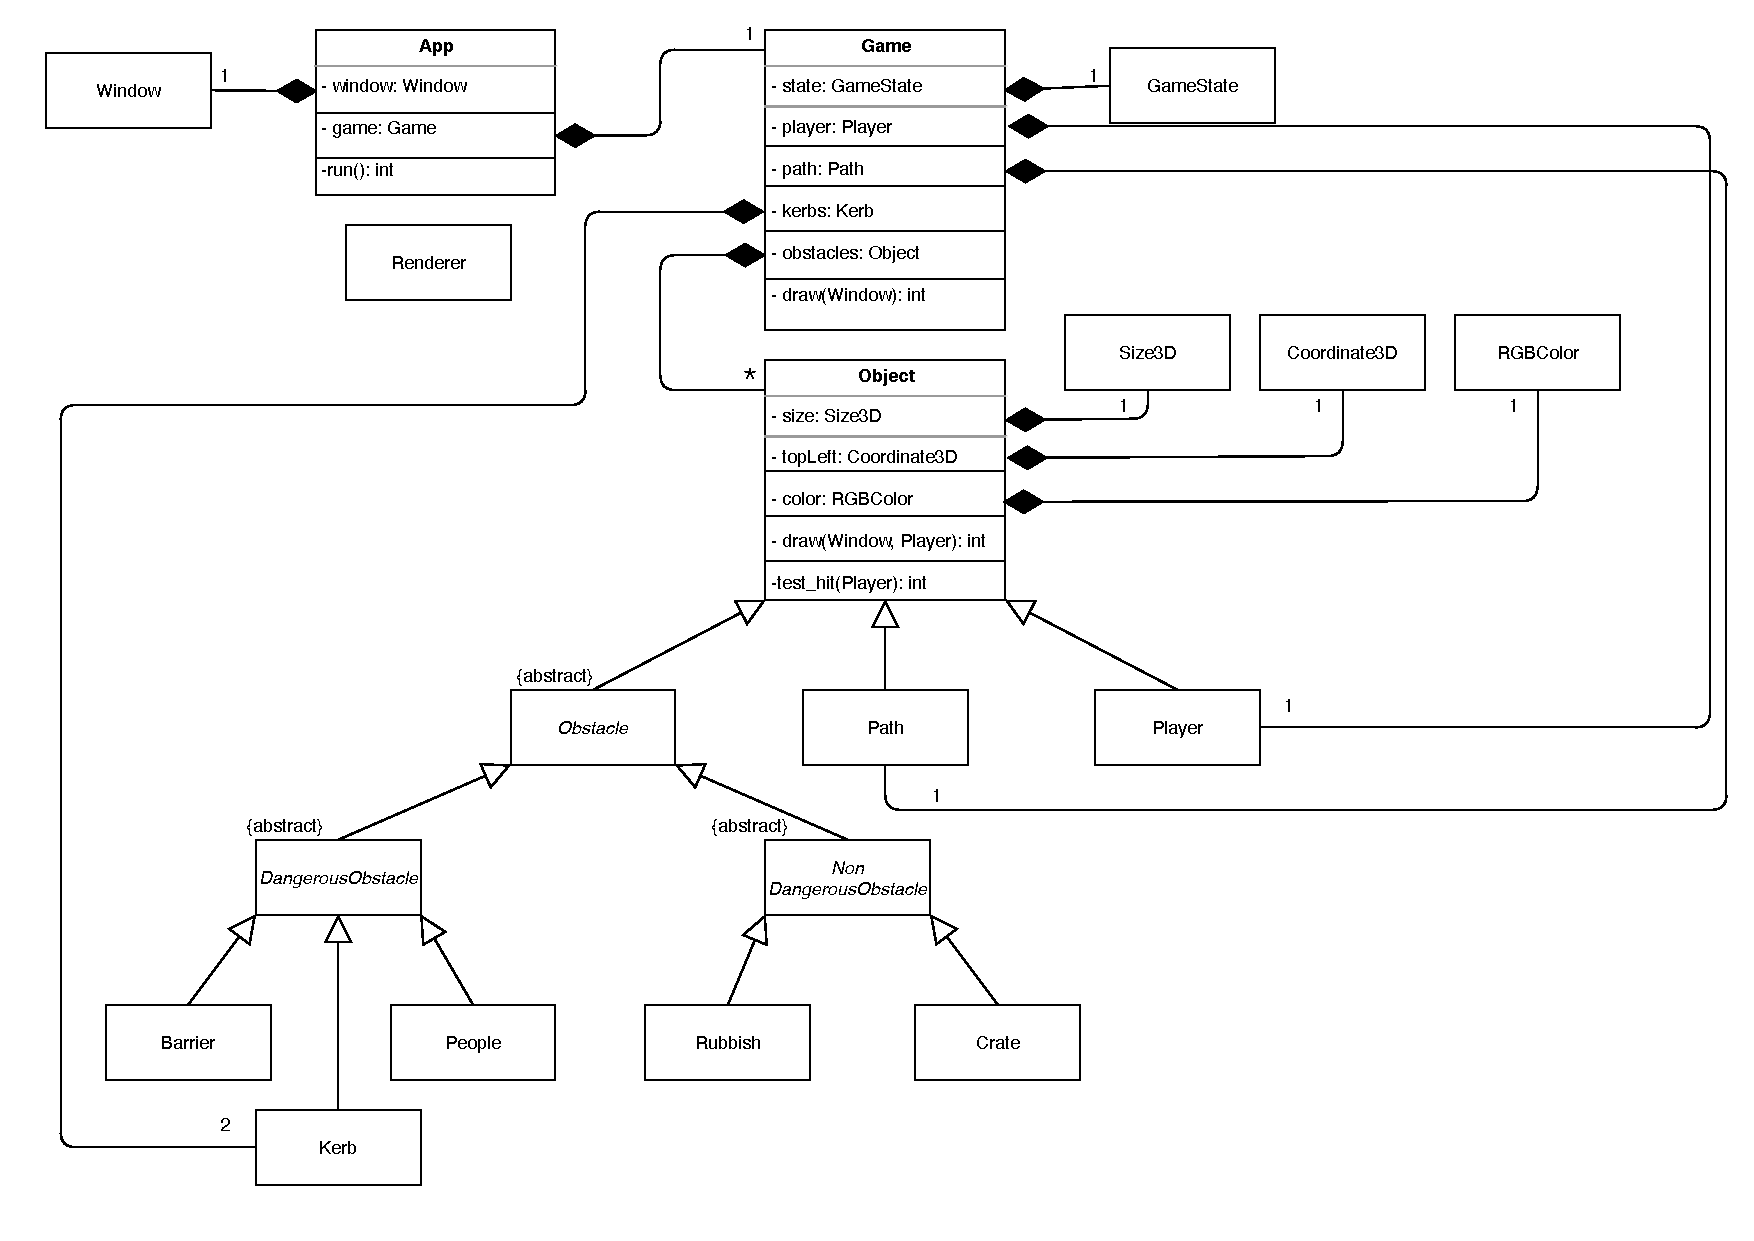
\includegraphics[width=1.2\textwidth]{uml.pdf}}%
  \caption{UML static diagram}
\end{figure}
\paragraph{}The class \texttt{Window} is a wrapper around a \texttt{SDL\_Window} which stores some information about the window it is representing as long as a few functions that are wrappers around SDL functions. These functions allow to draw a line, a rectangle, or a text on the window.\\ \newline
The class \texttt{App} represents the application. It is responsible for running the game, handling the events, and quitting the game properly at the end.\\ \newline
The goal of the class \texttt{Renderer} is to compute the coordinates of the perspective of a given point and to calculate the coordinates of the point on the window coordinate system.\\ \newline
The class \texttt{Game} is representing the game. It is responsible for the logic of the game and for maintaining references to all the elements needed by the game. It has a lot of responsibilities with the most important being to draw the game on a given window, test if the player hit something, and generating random obstacles.\\ \newline
The class \texttt{GameState} is responsible for maintaining the state of the ongoing game. It is remembering if the game is still ongoing and the distance travelled by the player.\\ \newline
The class \texttt{Object} represents every object of the game. It stores information about an object, including its size, position, and color. These properties are respectively represented by the class \texttt{Size3D}, \texttt{Coordinate3D}, and \texttt{RGBColor}. It also has a function to draw the object on a given window and another one to test if the player hit the object.\\
The class \texttt{Path} represents the path on which the player is walking.\\ \newline
The class \texttt{Player} represents the player (Cymi) of the game.\\ \newline
The abstract class \texttt{Obstacle} represents every obstacle of the game. It is further divided into \texttt{DangerousObstacle} and \texttt{NonDangerousObstacle} which respectively represent obstacles on which the player will trip and obstacles on which it will not trip.\\ \newline
The class \texttt{DangerousObstacle} is itself specialized into \texttt{Barrier}, which represents a barrier, \texttt{People}, which represents a person standing on the path, and \texttt{Kerb}, which represents a kerb on the side of the path.\\ \newline
The class \texttt{NonDangerousObstacle} is also specialized in \texttt{Rubbish}, which represent a rubbish left by the people on the path, and \texttt{Crate}, which represent a crate on the path.

\paragraph{}Each class has two files associated to it. The names of the files associated to a given class are the name of the class then \texttt{.hpp} or \texttt{.cpp} depending on whether you are searching for the interface or the implementation of the class.


%%%%%%%%%%%%%%%%%%%%%%%%%%%%%%%%%%%%%%%%%%%%%%

\section{Design}
\paragraph{}In this section, we will present how we solved the non-obvious specific problems and justify these implementation choices.

\subsection{Obstacles generation}
\paragraph{}We generated our obstacles from the closest to the farthest and taking into account the applicate of the last generated obstacle. We chose to proceed like that in order to not have any overlap between two or more obstacles. Moreover, closest obstacles should be generated before farthest obstacles because there are the first ones visible by the player.
\paragraph{}These obstacles were generated according to the proportions of dangerous and non-dangerous obstacles that can be easily modified in our code.

\subsection{Coordinates projection}
\paragraph{}To draw the elements of our game, we had to project their 3D coordinates, that we were storing in centimeters in memory, to their perspective 2D coordinates in pixels. This task was not really hard thanks to the formula given in the statement. We just had to take the field of view into account using some right triangles trigonometry formula and then passing from centimeters to pixels using the computed scaling factors. Finally, we had to translate the computed coordinates to the window coordinate system.
\paragraph{}We chose to store 3D coordinates using centimeters as units because it was easier to manipulate than pixels. All the necessary computations for these projections are implemented in the \texttt{Renderer} class. 

\subsection{Drawing of obstacles}
\paragraph{}We drawn the obstacles, which are all rectangular parallelepipeds, from back to front because back obstacles are hidden by front obstacles mimicking the real-life view. 
\paragraph{}Moreover, the points representing an obstacle were drawn from back to front for the same reason. Front and back faces were drawn by drawing rectangles, while side faces were drawn line by line with an increasing applicate.

\subsection{Collision detection}
\paragraph{}The player and obstacles being all rectangular parallelepipeds, the detection of collisions consists of, at each move, taking the player and the sizes of the obstacles and checking if one point inside an obstacle box is also inside the player box. We chose to detect collisions this way because we found that it was the more natural way of detecting such collisions.

%%%%%%%%%%%%%%%%%%%%%%%%%%%%%%%%%%%%%%%%%%%%%%

\section{Feedback about the assignment}
\paragraph{}In this section, we will explain the main difficulties we encountered during the development of this project as long with an approximation of the time we spent on this project.
\paragraph{}Undoubtedly, the hardest part was the rendering process. We encountered some troubles to take the field of view into account when drawing the obstacles on the window. The other parts of the project were not that hard once we had our architecture figured out.
\paragraph{}Regarding the time we spent, we both spent approximately 15 hours on the project.

%%%%%%%%%%%%%%%%%%%%%%%%%%%%%%%%%%%%%%%%%%%%%%

\end{document}
